\section{Adjacency spectral embedding}
\label{sec:ch6:ase}

\begin{floatingbox}[h]\caption{Give $SBM_n(\vec z, B)$ random networks and linear algebra a revisit}
In this section, we're going to revisit the $SBM_n(\vec z, B)$ random networks. The intuition that you gained in \ref{sec:ch5:psd_block} will be critical for the embedding approach that we learn here, so give it another read. 

The key algorithms that we will use in this section are known as the {eigendecomposition} and the {singular value decomposition}. To situate yourself in the process for the {eigendecomposition}, we would recommend that you look at \cite{Axler}. To situate yourself in the process for the singular value decomposition \cite{Trefethen1997}, lectures 1 through 4. This covers all of the basic intuition that you will need to remember about the \textit{eigendecomposition}, the singular value decomposition, and will get you back in the mindset of matrix multiplication, which will be a key result that we will need here.
\end{floatingbox}

Let's imagine that we have a probability matrix $P$ for a simple indepndent-edge random network which is positive semi-definite. Remember that for a positive semi-definite real matrix, the square-root matrix exists and is real, which we explored in Section \ref{sec:ch5:psd_block}. 

If we let $X = \sqrt{P}$ be the square-root matrix for $P$, this means that $P$ is the probability matrix corresponding to an $RDPG_n(X)$ random network. For our purposes, we will assume that the network has $n$ nodes, and $X$ has a latent dimensionality of $d$ which is less than the number of nodes, and that none of the columns are redundant (the rank of $X$ is $d$).

\subsection{The eigendecomposition provides us with latent position matrices for random networks with positive semi-definite probability matrices}


Since the network is simple, $P$ is symmetric, as simple networks are undirected. Finally, as we learned in Section \ref{sec:ch5:ier:ier_generalises}, matrices that can be expressed as the product of a real matrix and its transpose are positive semi-definite, so $P$ is positive semi-definite (since it is $X$ times its transpose).

These facts provide us with a number of useful implications about the eigendecomposition of $P$, in Remark \ref{box:ch6:evd_sum}.
\begin{floatingbox}[h]\caption{The eigendecomposition of symmetric matrices}
\label{box:ch6:evd_sum}
If $R$ is a real symmetric square matrix with real entries, then the \textit{eigendecomposition} of $R$ is the factorization $R = Q\Lambda Q^\top$ where $\Lambda$ is the diagonal matrix of the ordered (in decreasing order) eigenvalues of $P$, and $Q$ is the matrix whose columns are eigenvectors of $P$. 

If $R$ is rank $d$, $\Lambda$ will have $d$ eigenvalues that are non-zero, and the remaining $n - d$ eigenvalues will be $0$. 

If $R$ is positive semi-definite, the eigenvalues will further be non-negative; so, $\lambda_1 \geq \lambda_2 \geq \hdots \geq \lambda_ n \geq 0$.

If $R$ is both symmetric, positive semi-definite,and rank $d$, then combining these facts gives two key results:
\begin{enumerate}
    \item The non-zero eigenvalues are ordered and positive: $\lambda_1 \geq \hdots \lambda_d > 0$.
    \item with $Q_d$ the $n \times d$ matrix whose entries are the first $d$ eigenvectors of $P$, and $\Lambda_d$ the $d \times d$ diagonal matrix whose diagonal entries are the first $d$ non-zero eigenvalues of $R$:
\begin{align*}
R = Q_d \Lambda_d Q_d^\top
\end{align*}
\end{enumerate}
Throughout this book, we notate the eigendecomposition of a matrix $R$ with $\texttt{evd}(R)$.
\end{floatingbox}

So, if $P$ is positive semi-definite, rank $d$, and symmetric, this allows us to obtain a characterization of the latent positions of $P$, where we can obtain that:
\begin{align*}
    P = YY^\top,\;\;\;\; Y = Q_d \sqrt{\Lambda_d}
\end{align*}
where $\sqrt{\Lambda_d}$ is the matrix whose entries are the square roots of the first $d$ eigenvalues of $P$. Note that $\sqrt{\Lambda_d}$ is real, because the top $d$ eigenvalues are positive, so their square root is defined. We can put this entire procedure together, using Algorithm \ref{alg:ch6:evd}, to obtain a latent position matrix for the random network.

\begin{algorithm}[h]\caption{Finding latent positions for a positive semi-definite probability matrix}
\label{alg:ch6:evd}
\KwData{$P$ a $n \times n$ square probability matrix which is positive semi-definite and of rank $d$.}
\KwResult{a latent position matrix for the random network.}
\SetAlgoLined
Let $Q, \Lambda = \texttt{evd}(P)$ be the eigenvectors and eigenvalues of $P$.

Let $Q_d = \begin{bmatrix}
    \uparrow & & \uparrow \\
    \vec q_1 & \hdots & \vec q_d \\
    \downarrow & & \downarrow
\end{bmatrix}$, and let $\Lambda_d = \begin{bmatrix}
    \lambda_1 & & \\
    & \ddots & \\
    & & \lambda_d
\end{bmatrix}$ be the matrix whose rows are the first $d$ eigenvectors and the diagonal matrix whose entries are the first $d$ eigenvalues of $P$.

Compute $\sqrt{\Lambda_d}$ to be the matrix whose entries are $\sqrt{\lambda_i}$, for all $i$ from $1$ to $d$.

Let $Y = Q_d \sqrt{\Lambda_d}$.

\Return{$Y$}
\end{algorithm}

This gives us a method to compute a latent position matrix for the underlying random network, which has $n$ rows and $d$ columns. 


\subsubsection{Rotational non-identifiability of the latent position matrix}
\label{sec:ch6:spectral:nonidentifiable}
As it turns out, there are many ``reasonable'' latent position matrices for a random network with a positive semi-definite probability matrix, where by ``reasonable'', we mean that they all would produce the same latent position matrix. In particular, there are infinitely many embeddings that are identical up to a rotation.

A \textit{rotation matrix} $W$ in $d$-dimensions is any $d$-dimensional matrix where $WW^\top = W^\top W = I_d$, the $d$-dimensional identity matrix.

Let's imagine that $X$ is another latent position matrix, but is a rotation of $Y$. That means that there is a rotation matrix $W$ where $X = YW$. The probability matrix for the $RDPG_n(X)$ network is:
\begin{align*}
    P &= XX^\top \\
    &= YW\left(YW\right)^\top,
\end{align*}
which is because $X = YW$. Applying the definition of a transpose, we get:
\begin{align*}
    P &= YW W^\top Y^\top \\
    &= YI_d Y^\top,
\end{align*}
which is because $W$ was a rotation matrix, so $W^\top W = WW^\top = I_d$. Finally, since $YI_d = Y$ (by definition of the identity matrix):
\begin{align*}
    P &= YY^\top.
\end{align*}
This shows that the $RDPG_n(Y)$ and $RDPG_n(X)$ random networks have the same probability matrices.

This is known as the \textit{rotational non-identifiability} problem with random dot product graphs, in that random networks with different latent position matrices (by as much as an arbitrary rotation by the rotation matrix $W$) can still have the same probability matrix. Therefore, different latent position matrices can describe fundamentally identical (in probability) random networks.

\subsubsection{Limitations of the \texttt{evd} for adjacency matrices}

These results are helpful when we know the probability matrix ahead of time. In fact, we even know how to determine whether the probability matrix is positive semi-definite, using the procedure that we developed in Section \ref{sec:ch5:psd_block}, where we simply checked whether all of the eigenvalues were non-negative.


Unfortunately, in real data, we don't typically have the probability matrix; all that we have is the network itself. This network can typically be represented in an adjacency matrix. 

It would be helpful (and maybe even intuitive) if we could simply plug in the adjacency matrix into Algorithm \ref{alg:ch6:evd}, and obtain a reasonable estimate of the latent positions out. While this matrix is real and symmetric, it is unfortunately not necessarily positive semi-definite.

Consider, for instance, an extremely simple network you might obtain:
\begin{align*}
    A &= \begin{bmatrix}
        0 & 1 \\
        1 & 0
    \end{bmatrix}
\end{align*}
Remember that for a $2 \times 2$ matrix to be positive semi-definite, a characterization from Section \ref{sec:ch5:psd_block} was that $det(A) \geq 0$. However, $det(A) = 0 \cdot 0 - (1 \cdot 1) = -1$, so this matrix is not positive semi-definite. 

This means that none of the logical basis that led to the conclusion of Algorithm \ref{alg:ch6:evd} applies to adjacency matrices; for instance, in this simple example, the matrix $\sqrt{\Lambda_d}$ is not even a real matrix (it is a complex matrix, since $\sqrt{-1} = i$). 

In practice, the implications of this trivial example are that we cannot use the eigendecomposition to obtain real estimates of latent position matrices from adjacency matrices.

\subsection{The singular value decomposition allows us to estimate latent positions}

There is a closely related approach, the \textit{singular value decomposition}, which we can use as a logical basis to obtain a real estimate of latent position matrices. We summarize many useful results about the singular value decomposition in Remark \ref{box:ch6:svd}.

\begin{floatingbox}[h]\caption{The singular value decomposition of real matrices}
\label{box:ch6:svd_results}
If $R$ is a real square matrix of rank $d$, then the \textit{singular value decomposition} is the factorization $P = U\Sigma V^\top$, where $\Sigma$ is the diagonal matrix of the non-negative ordered \textit{singular values} of $P$, $U$ is an orthonormal matrix whose $n$ columns $\vec u_i$ are the $n$-dimensional \textit{left singular vectors} of $R$, and $V$ is an orthonormal matrix whose $n$ columns $\vec v_i$ are the $n$-dimensional \textit{right singular vectors} of $R$. 

If $R$ is rank $d$, $\Sigma$ will have $d$ singular values that are non-zero, and the remaining $n - d$ singular values will be $0$.

If $R$ is positive semi-definite, then all left and right singular vectors $\vec u_i = \vec v_i$ for any $\sigma_i > 0$. This implies that for positive semi-definite $R$:
\begin{align*}
    R &= U \Sigma U^\top,
\end{align*}
and further if $R$ is rank $d < n$, with $U_d$ the $n \times d$ matrix of the top $d$ left singular vectors of $U$ and $\Sigma_d$ the $d \times d$ diagonal matrix of the top $d$ singular values:
\begin{align*}
    R &= U_d \Sigma_d U_d^\top.
\end{align*}

Throughout this book, we notate the singular value decomposition of a matrix $R$ with $\texttt{svd}(R)$. 
\end{floatingbox}

This allows us to obtain a closely related characterization of the latent positions of $P$, where:
\begin{align*}
    P &= YY^\top,\;\;\;\;Y = U_d \sqrt{\Sigma_d} \numberthis \label{eqn:ch6:ase_probmtx}
\end{align*}
where $\sqrt{\Sigma_d}$ is the matrix whose entries are the square-roots of the first $d$ singular values of $P$, and $U_d$ are the first $d$ left singular vectors of $P$. 

The equality here requires the positive semi-definiteness of $P$, that $P$ is rank $d$, and that $P$ is symmetric.

However, there is a convenient caveat: the matrices $U$ and $V$ are by definition real matrices for any real matrix $R$. Further, the eigenvalues $\sigma_i$ are necessarily non-negative, which means that they have a square root which is real. This gives us a basis for the procedure in Algorithm \ref{alg:ch6:ase}. Unlike the procedure described in Algorithm \ref{alg:ch6:evd}, the procedure of Algorithm \ref{alg:ch6:ase} where $\hat Y = \texttt{ase}(A)$ will always produce a real estimate of a latent position matrix. 

\begin{algorithm}[h]\caption{Estimating latent positions from adjacency matrices (\texttt{ase})}
\label{alg:ch6:ase}
\KwData{$A$ an adjacency matrix for a simple network.\newline $d$ a target latent dimensionality.}
\KwResult{an estimate of a latent position matrix.}
\SetAlgoLined
Let $U, \Sigma, V^\top = \texttt{svd}(A)$ be the left singular vectors, the singular values, and the right singular vectors of $A$.

Let $U_d = \begin{bmatrix}
    \uparrow & & \uparrow \\
    \vec u_1 & \hdots & \vec u_d \\
    \downarrow & & \downarrow
\end{bmatrix}$, and let $\Sigma_d = \begin{bmatrix}
    \sigma_1 & & \\
    & \ddots & \\
    & & \sigma_d
\end{bmatrix}$ be the matrix whose rows are the first $d$ left singular vectors and the diagonal matrix whose entries are the first $d$ singular values of $A$.

Compute $\sqrt{\Sigma_d}$ to be the matrix whose entries are $\sqrt{\sigma_i}$, for all $i$ from $1$ to $d$.

Let $\hat Y = U_d \sqrt{\Sigma_d}$.

\Return{$\hat Y$}
\end{algorithm}

This process is known as the Adjacency Spectral Embedding, or \texttt{ase}. It is called ``Adjacency'' because it operates on the adjacency matrix. ``Spectral'' just denotes that its theoretical intuition relies on the eigenvalues/eigenvectors of $P$ (the only reason that we calculated singular values/vectors of $A$ was for the convenience that it yielded a real matrix and not a complex one, and the properties for both approaches are similar). That it is an ``embedding'' simply denotes that it finds a mathematical structure contained in another (a tabular structure contained within the adjacency matrix, as explained in Remark \ref{box:ch6:tabularize}). 


\begin{floatingbox}[h]\caption{\texttt{ase} tabularizes your adjacency matrix}
\label{box:ch6:tabularize}
One of the challenges that we noted in Section \ref{sec:ch1:challenges} and reiterated in Section \ref{sec:ch6:why} was that network data fundamentally differs from traditional machine learning in that the data is not tabular. However, the embedding process has changed this for us: we have used a bag of nodes approach to tabularize the network into an real estimated latent position matrix with $n$ rows (one for each node) and $d$ columns (one for each latent dimension). This provides us with a tabular data structure, which we can build upon later on to explore the nodes using more traditional machine learning approaches. 
\end{floatingbox}


Let's make this a little more concrete with an example. Let's imagine that we have an $SBM_n(\vec z, B)$ with $100$ nodes, where the first $50$ nodes are in community $1$, and the second $50$ nodes are in community $2$. The block matrix will be homophilic, so by Section \ref{sec:ch5:psd_block}, the probability matrix is positive semi-definite.


\begin{lstlisting}[style=python]
from graspologic.simulations import sbm
from graphbook_code import generate_sbm_pmtx, lpm_from_sbm
import numpy as np

n = 100
# construct the block matrix B as described above
B = np.array([[0.6, 0.1], 
              [0.1, 0.4]])

# sample a graph from SBM_{100}(tau, B)
A, zs = sbm(n=[n//2, n//2], p=B, return_labels=True)

X = lpm_from_sbm(zs, B, zero_index=True)
P = generate_sbm_pmtx(zs, B, zero_index=True)
\end{lstlisting}

We show a plot of the latent positions, the probability matrix, and our network sample in Figure \ref{fig:ch6:ase:ex}. Notice that in this example, the latent positions are all equal for nodes from the same community. In light of the results we explored in Section \ref{sec:ch5:psd_block:same_lp}, this is as we would expect for an $SBM_n(\vec z, B)$ random network.

\begin{figure}
    \centering
    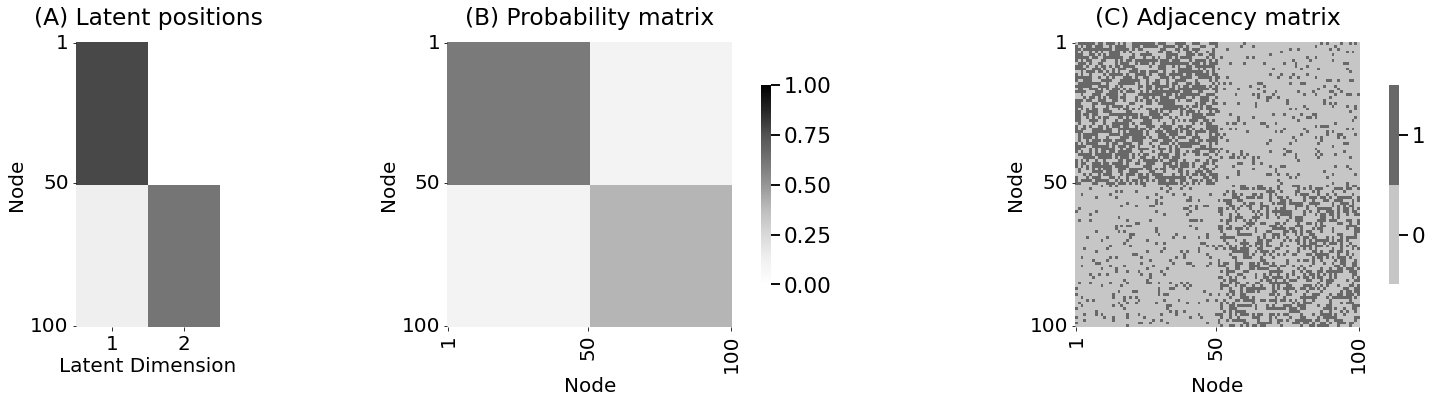
\includegraphics[width=\linewidth]{representations/ch6/Images/ase_sbm_ex.png}
    \caption[$SBM_n(\vec z, B)$ example for ASE]{\textbf{(A)} latent positions of the $SBM_n(\vec z, B)$ random network, \textbf{(B)} the probability matrix of the $SBM_n(\vec z, B)$ random network, \textbf{(C)} a sample of the $SBM_n(\vec z, B)$ random network.}
    \label{fig:ch6:ase:ex}
\end{figure}

Next, we use \texttt{graspologic} to compute the \texttt{ase} of our network sample. Note that we know that there are two communities here, so we embed into two dimensions. This gives us an estimate of the latent position matrix:

\begin{lstlisting}[style=python]
from graspologic.embed import AdjacencySpectralEmbed as ase

d = 2  # the latent dimensionality
# estimate the latent position matrix with ase
Xhat = ase(n_components=d).fit_transform(A)
\end{lstlisting}
Using this estimate of the latent position matrix, we can also visualize an estimate of the probability matrix, as:
\begin{align*}
    \hat P &= \hat X \hat X^\top.
\end{align*}
Let's do this with numpy:

\begin{lstlisting}[style=python]
Phat = Xhat @ Xhat.transpose()
\end{lstlisting}
We plot the estimated latent position matrix and probability matrix in Figure \ref{fig:ch6:ase:est}(A) and (B), and the true latent position matrix and probability matrix in Figure \ref{fig:ch6:ase:est}(C) and (D).

In the example when we ran it, the estimated latent positions $\hat X$ look really similar to the true latent positions $X$. However, due to the fact that there is some randomness in how the \texttt{svd} algorithm is implemented in \texttt{numpy}, this won't always be the case, due to the non-identifiability issue that we noted in Section \ref{sec:ch6:spectral:nonidentifiable}. This means that your latent positions might be rotated around.

Regardless of rotational issues, you should see that the estimated probability matrix $\hat P$ should be fairly similar to the true probability matrix $P$.

\begin{figure}[h]
    \centering
    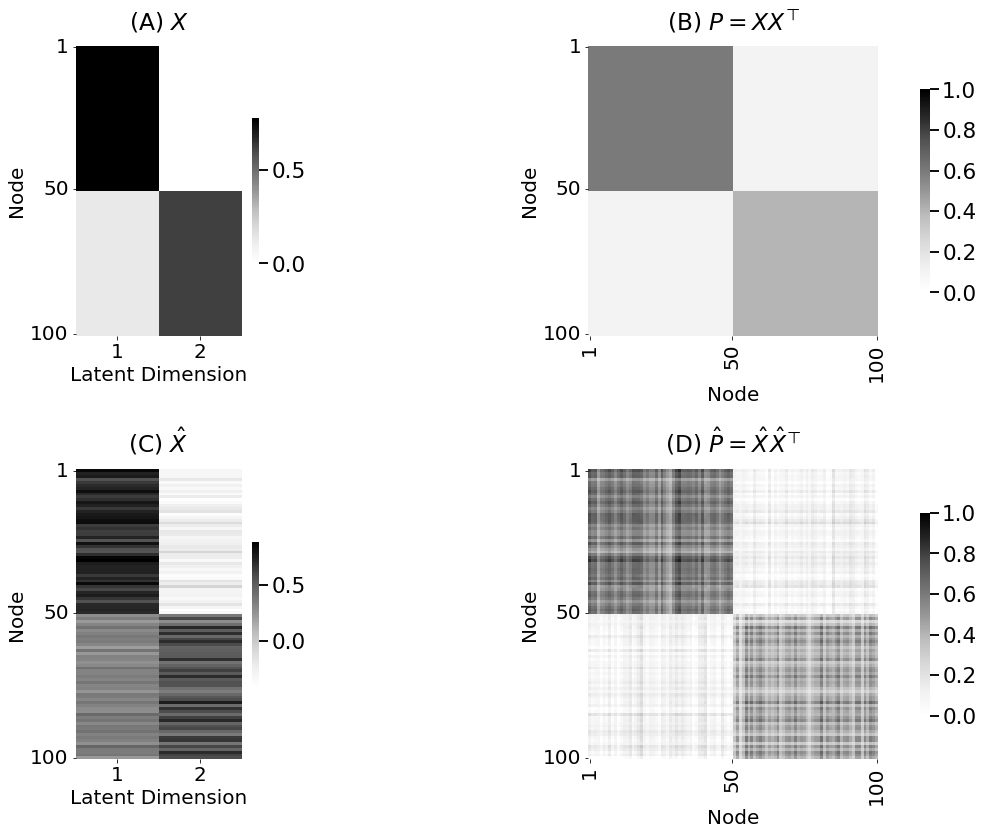
\includegraphics[width=0.7\linewidth]{representations/ch6/Images/ase_result.png}
    \caption[Comparison of ASE estimate to true prob. matrix]{\textbf{(A)} the true latent positions, \textbf{(B)} the true probability matrix, \textbf{(C)} the estimated latent positions, \textbf{(D)} the estimated probability matrix.}
    \label{fig:ch6:ase:est}
\end{figure}

Since we know the community labels of our network ahead of time, this pattern that you observe is pretty obvious. In particular, the first $50$ nodes (community $1$) tend to have similar latent position vectors, and the second $50$ nodes (community $2$) tend to have similar latent position vectors. In light of Section \ref{sec:ch5:psd_block:same_lp}, this intuitively should make sense to you: the true latent positions are {identical} for nodes in the same community, so it makes sense that the estimated latent positions will be at least close.

Now, let's consider what happens when we randomly reorder the nodes of the network, just like we did in Section \ref{sec:ch5:sbm:modularity}:

\begin{lstlisting}[style=python]
vtx_perm = np.random.choice(n, size=n, replace=False)

# reorder the adjacency matrix
Aperm = A[tuple([vtx_perm])] [:,vtx_perm]
# reorder the community assignment vector
zperm = np.array(zs)[vtx_perm]

# compute the estimated latent positions using the
# permuted adjacency matrix
Xhat_perm = ase(n_components=2).fit_transform(Aperm)
\end{lstlisting}
Now, our adjacency matrix looks like Figure \ref{fig:ch6:ase:ase_permuted}(A), and the estimated latent positions look like Figure \ref{fig:ch6:ase:ase_permuted}(B). It's not quite as obvious now that two pairs of $50$ nodes in the network have similar latent positions looking solely at the heatmap of $\hat X$ in (B), because these groups of nodes have been dispersed throughout the network. 

\begin{figure}
    \centering
    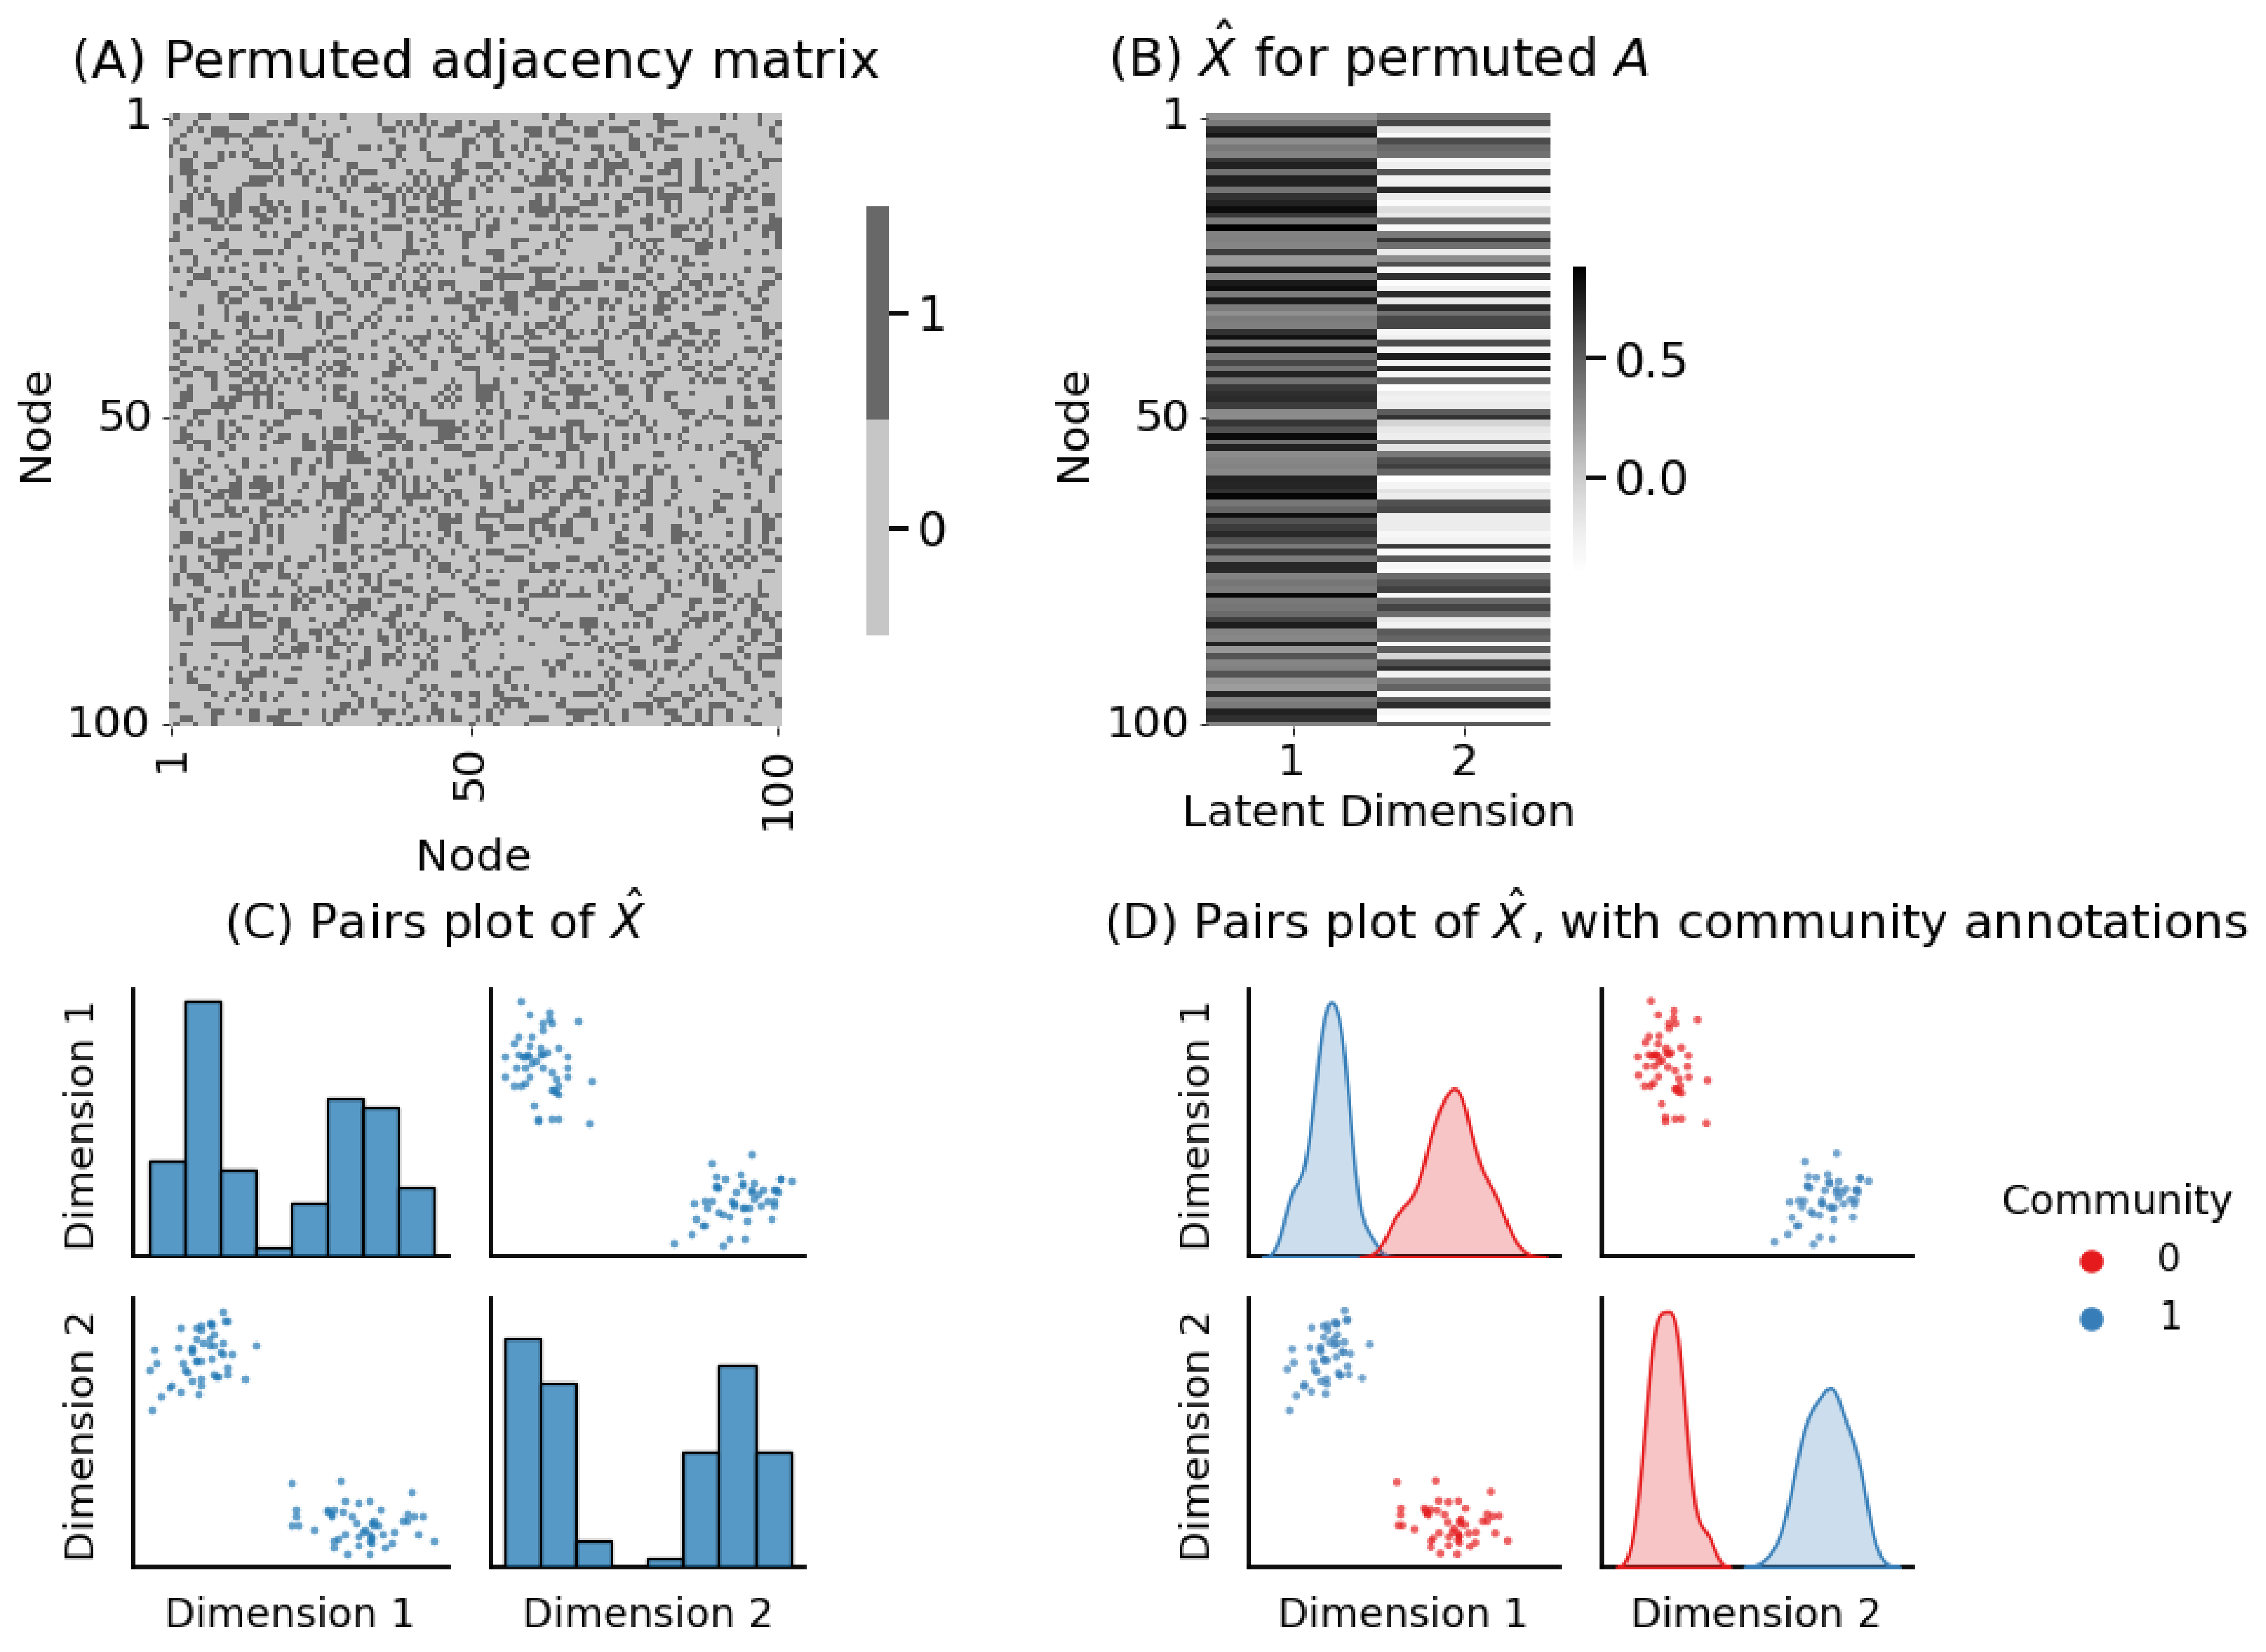
\includegraphics[width=\linewidth]{representations/ch6/Images/ase_permuted.png}
    \caption[ASE recovers latent structure, permutation-agnostic]{\textbf{(A)} the permuted adjacency matrix, \textbf{(B)} the estimated latent positions of the permuted adjacency matrix. \textbf{(C)} the pairs plot of the estimated latent positions of the permuted adjacency matrix, and \textbf{(D)} the pairs plot shown with the true community labels of the nodes.}
    \label{fig:ch6:ase:ase_permuted}
\end{figure}

\subsubsection{The ``pairs plot'' for estimated latent positions}
\label{sec:ch6:ase:reorder}
One way to visualize tabular data structures is to use something called a ``pairs plot'', which you may have come across in machine learning. With a pairs plot, you visually investigate tabular data for \textit{latent structure}; that is, you to look for patterns that are hidden in a dataset.

To study the pairs plot, you can simply call the pairs plotting utility directly from graspologic:

\begin{lstlisting}[style=python]
from graspologic.plot import pairplot

fig = pairplot(Xhat, title="Pairs plot of $\\hat X$")
\end{lstlisting}

The pairs plot for the estimated latent positions is shown in Figure \ref{fig:ch6:ase:ase_permuted}(C). The pairs plot is a d x d matrix of plots, where d is the total number of features of the matrix for which a pairs plot is being produced. The plot is called a ``pairs'' plot because it plots “pairs” of dimensions. Notice that there are two distinct looking ``blobs'' of point clouds in the pairs plot of $\hat X$.

For each off-diagonal plot (the scatter plots), the $k^{th}$ row and $l^{th}$ column scatter plot has the points $(x_{ik}, x_{il})$ for each node in the network. Stated another way, the off-diagonal plot is a scatter plot for each node of the $k^{th}$ dimension and the $l^{th}$ dimension of the matrix being plotted. That these scatter plots indicate that the points appear to be separated into individual clusters provides evidence that there might be latent community structure in the network. It is pretty clear that this plot is symmetric, since the off-diagonal entries are simply mirror images of one another (one will be dimension $k$ against dimension $l$, and the off-diagonal entry will be dimension $l$ against dimension $k$).

The diagonal elements of the pairs plot simply represent histograms or density estimates (called \textit{Kernel Density Estimates}, or KDEs) of the estimated latent positions for each dimension. If you do not pass in labels, you obtain histograms, which are just scaled bins which show the number of points for a given dimension which fall into the indicated range. If you do pass in labels, you obtain density estimates, where higher densities indicate that more points have latent position estimates in that range. For instance, the top-left density estimate indicates a density estimate of the first latent dimension for all nodes, the middle is a density estimate of the second latent dimension for all nodes, so on and so forth.

When the number of embedding dimensions is two, showing a full pairs plot is redundant, so we will often simply show a scatter plot of dimension $1$ against dimension $2$ for two-dimensional settings.

Now, let's see what happens to the pairs plot for $\hat X$, which we pass in the community labels for the nodes:

\begin{lstlisting}[style=python]
fig = pairplot(Xhat_reordered, labels=zperm, legend_name = "Community",
             title="Pairs plot of randomly reordered $\\hat X$")
\end{lstlisting}

The resulting plot is shown in Figure \ref{fig:ch6:ase:ase_permuted}(D). Now we're getting somewhere! It looks like these two distinct ``blobs'' that we noticed in (C) each correspond to a single community in the underlying $SBM_n(\vec z, B)$ random network. In fact, nodes of the same community will tend to have estimated latent positions that are close together. When we say the vectors are ``close together'', what we really are talking about is with respect to the Euclidean distance. The Euclidean distance is:

\begin{floatingbox}[h]\caption{Euclidean distance between two vectors}
\label{def:ch6:se:eucl_dist}

If $\vec x = (x_i)_{i = 1}^d$ and $\vec y = (y_i)_{i = 1}^d$ are two $d$-dimensional real vectors, the \textit{Euclidean distance} is defined as:
\begin{align*}
    d(\vec x, \vec y) = \|\vec x - \vec y\|_2 = \sqrt{\sum_{i = 1}^d (x_i - y_i)^2}.
\end{align*}
\end{floatingbox}
To evaluate this, we can compute the distance matrix of the estimated latent positions, $D$. We'll rotate back to the unpermuted points for this plot, just to make the intuitive connection more immediate. Each entry $D_{ij}$ corresponds to the distance $d(\hat{\vec x}_i, \hat{\vec x}_j)$ between all pairs of estimated latent positions. We can compute the pairwise distance matrix using \texttt{scipy}:

\begin{lstlisting}[style=python]
from scipy.spatial import distance_matrix

D = distance_matrix(Xhat, Xhat)
\end{lstlisting}
A plot of the pairwise distance matrix is shown in Figure \ref{fig:ch6:ase:nonidentifiable}(A). Note that the pairwise distance matrices between the first $50$ nodes (community $1$, the upper-left block of the pairwise distance matrix) and the second $50$ nodes (community $2$, the bottom-right block of the pairwise distance matrix) are relatively small, but the pairwise distances between nodes from community $1$ and nodes from community $2$ (and vice-versa, in the upper-right and bottom-left blocks of the pairwise distance matrix) are relatively large.

This will be extremely useful to us in Section \ref{sec:ch7:comm_detect} when we attempt to estimate underlying community structure from $SBM_n(\vec z, B)$ random networks.

\subsubsection{Rotational non-identifiability and the estimated latent positions}

As we mentioned in Section \ref{sec:ch6:spectral:nonidentifiable}, the latent positions are rotationally non-identifiable, in that for an $RDPG_n(X)$ with latent positions $X$, an $RDPG_n(XW)$ where $W$ is a $d$-dimensional rotation matrix has the same probability matrix. The estimated latent positions $\hat X$ share this issue. Now that we have estimated latent positions, we can illustrate this with our example. 

Let's see what our original latent positions look like as a scatter plot (a plot of $\hat X$ similar to the pairs plot you learned about above), and then when we apply a rotation matrix $W$ to $\hat X$, such as if we rotate $\hat X$ by $90^\circ$ to the right:

\begin{lstlisting}[style=python]
# a rotation by 90 degrees
W = np.array([[0, 1], [1, 0]])
Yhat = Xhat @ W

np.allclose(Yhat @ Yhat.transpose(), Xhat @ Xhat.transpose())
# returns True
\end{lstlisting}

As you can see in Figure \ref{fig:ch6:ase:nonidentifiable}, the estimated latent positions in (B) are basically the same in (C), except they are rotated by $90^\circ$ to the right. Note that the top blob has moved to the right, and the right blob has moved to the bottom. This is one particular example of a rotation, but there are infinitely many rotations we could make for our $2$-dimensional latent position matrix.

\begin{figure}[h]
    \centering
    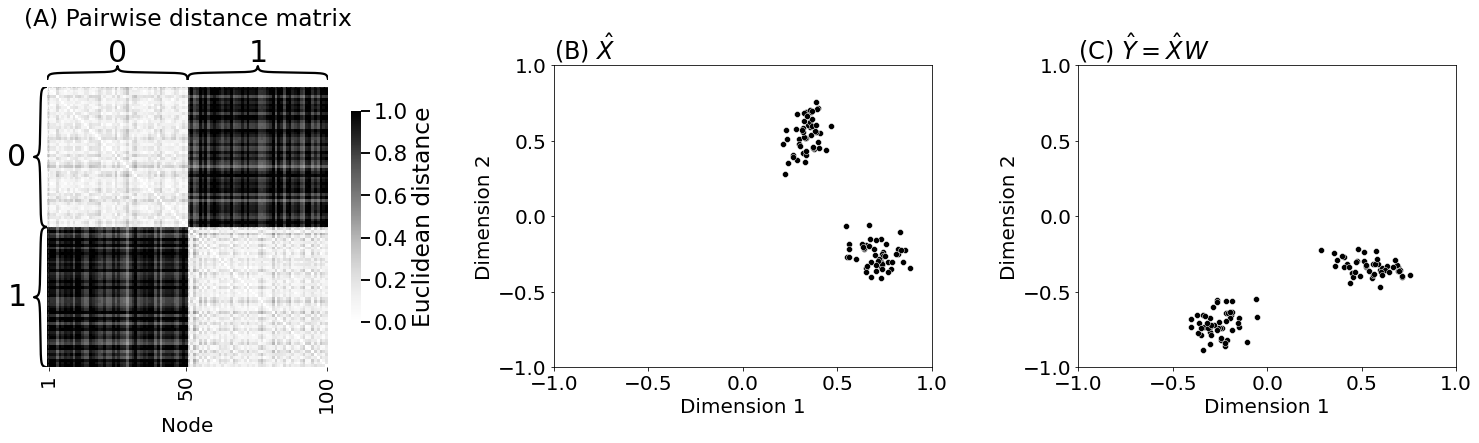
\includegraphics[width=\linewidth]{representations/ch6/Images/rotation.png}
    \caption[Pairwise distance matrices for latent positions]{\textbf{(A)} the pairwise distance matrix between the latent position vectors of all pairs of nodes, \textbf{(B)} the estimated latent positions, \textbf{(C)} the estimated latent positions, but rotated by $90^\circ$.}
    \label{fig:ch6:ase:nonidentifiable}
\end{figure}


\subsection{Why do we use \texttt{ase}?}
\label{sec:ch6:ase:whyuse}
At a very high level, the utility of \texttt{ase} is that it tabularizes your adjacency matrix, into an $n \times d$ real matrix, where $d$ was the number of dimensions that you selected to embed into. This provides the utility that you can learn about the nodes of your network via traditional machine learning approaches by treating the rows of the resulting matrix $\hat X$ as observations, and the columns of the matrix $\hat X$ as features. 

By now, we are ready to explore at a high level three additional reasons that we turn to \texttt{ase}:

\paragraph*{It always finds the latent positions for the probability matrix, given the latent dimensionality}

If you conceptualize your network sample as being a sample from an $IER_n(P)$ random network where the probability matrix is positive semi-definite, the procedure that you are using on the adjacency matrix is the same procedure that could operate on the underlying probability matrix and find the latent positions of it exactly (up to a rotation). \texttt{ase} was able to do this even if the underlying matrix was not positive semi-definite, so we would always obtain a real matrix (when we use something like an adjacency matrix).

\paragraph*{\texttt{ase} decouples the dependencies of the random network}

Studying $Y$ is equivalent (statistically) to studying $P$ when $P$ is a function of $Y$, such as $P = YY^\top$. Since $Y$ is far simpler than $P$ (it will usually have fewer columns, in practice), it will be easier to study, too.

Remember that a major limitation that we mentioned in Section \ref{sec:ch6:why} was that, for a random network $\mathbf A$, the dependency structure was simply too complicated to think about. This was because edges of the network were inherently coupled to the nodes of the network, suggesting that there were a number of possible dependencies on the order of $\frac{n!}{2}$ in the network (which was a really big number).

The probability matrix $P$ determines the structure of the random network $\mathbf A$, so we can study the probability matrix $P$ to gain insights about the dependencies in $\mathbf A$. If $P$ is positive semi-definite and $P = YY^\top$ for a set of latent positions, it is the case that the dependency structure encoded by $P$ is also encoded by $Y$. This means that the latent positions, which often will have a number of columns that is less than the number of nodes, encode the complicated dependency structure of the underlying network.

If the number of latent dimensions is less than the number of nodes in the network, that the number of possible dependencies that we will have to explore will be far less when we study the latent positions than when we study the random network (via the probability matrix) itself. 

\paragraph*{Estimated latent positions from \texttt{ase} are directly related to latent positions of random networks}

Most of the details that we have we have used thus far to conceptualize \texttt{ase} as a reasonable strategy deal with the spectral embedding of the probability matrix $P$, and the true underlying latent positions of the probability matrix (up to a rotation). We don't have this matrix $P$ in practice; we only have $A$. 

As long as we are comfortable with assuming that $A$ is a sample from a random network $\mathbf A$ with probability matrix $P$, there is theoretical reason to do this, too. ``Assuming that $A$ is a sample from a random network $\mathbf A$'' very loosely means that it makes sense to think that there was some level of randomness to the network sample. In light of the fact that most network samples are imperfect, which we explored in Section \ref{sec:ch1:howstudy}, this is not a major conceptual stretch to make.

Under this assumption, the estimates of latent positions $\hat Y$ will closely approximate the true latent positions $Y$ (up to a rotation) of $\mathbf A$ as the number of nodes in the network increases \cite{Sussman2012Sep,Athreya2017Jan,Rubin2022Sep}, and the estimate of the probability matrix $\hat P$ will closely approximate the true probability matrix $P$ (with no qualifications needed about rotations, due to the potential rotation of $\hat Y$ being ``cancelled out'' when we compute the probability matrix, like we saw in Section \ref{sec:ch6:spectral:nonidentifiable}). This is good news for us; it makes intuitive sense for estimates to be better and better approximates (on average) of the things they are approximating when we see more and more data. The theoretical advantages of \texttt{ase} are studied in detail in Appendix \ref{app:ch13:spectral}. 

There is an asterisk that will come up in a particular set of problems in which this does not hold, known as sparse networks, which will be discussed in Section \ref{sec:ch7:sparse}.

In the context of your work, what this means is that if conceptualizing your network as a sample of a random network with a positive semi-definite probability matrix feels appropriate, studying $\hat Y$ will be a good surrogate to use in place of studying $Y$ (since you can't obtain $Y$ from a network adjacency matrix $A$). This is powerful because the set of $IER_n(P)$ random networks where the probability matrix is positive semi-definite include many complicated structures, such as those shown in Section \ref{sec:ch5:psd_block}, and extensions of these structures to more than two communities. In fact, even outside of positive semi-definite structures, \texttt{ase} is still a reasonable strategy as we discuss briefly in Section \ref{sec:ch6:dimest:grdpg}. This approach therefore generalizes readily to a plethora of network learning problems. 

\subsection{Linear Algebra Considerations}

There is a lot of linear algebra that can help you build the intuition that you need to understand Remarks \ref{box:ch6:evd_sum} and \ref{box:ch6:svd_results}. We pulled this into Appendix \ref{app:ch13:ase}.

\newpage